\documentclass[10pt,a4paper]{article}

\usepackage{datetime}
\usepackage{numprint}
\usepackage{palatino}
\usepackage{authblk}
\usepackage[margin=0.75in]{geometry}
\usepackage{hyperref}
\usepackage{graphicx}
\usepackage{titlesec}
\usepackage{listings}
\usepackage{markdown}
\usepackage[english]{babel}
\usepackage[
	backend=biber,
	style=numeric,
]{biblatex}
\addbibresource{refs.bib}

\hypersetup{%
    pdfborder = {0 0 0}
}

\setlength{\parindent}{2em}
\setlength{\parskip}{1em}
\renewcommand{\baselinestretch}{1.0}

\begin{document}

\nplpadding{2}

\title{Malware Analysis Report: ``FritzFrog''\\ \vspace{-8pt} {\large CAP6137 Malware Reverse Engineering: P0x04}}
\author{{Naman Arora \\ \vspace{-10pt}\small \href{mailto:naman.arora@ufl.edu}{naman.arora@ufl.edu}}}
\date{\today}

\maketitle
\newpage
\tableofcontents
\newpage
\section{Executive Summary}
The malware sample provided has been identified to belong to \textit{FritzFrog} family of trojans/bot-nets.
It uses \textit{SSH} brute-force techniques to inject itself into the target machine.
Once injected, it opens up a listening port on the machine (\textit{Port 1234}) through which it enters into a \textit{peer-to-peer} swarm of similar victim bot-nets.
The communication between the individual bot-nets is encrypted and is routed through \textit{SSH tunnel}.
The bot-net uses an internal implementation of \textit{Database} to store peers' information, targets' information as well as binary data it collects.
A direct connection to a \textit{bot-master} could not be identified and thus, it is a strong indication that all the commands as well as data ex-filtration is done via a \textit{peer-to-peer} algorithm.
On analysis, it shows that the malware sample has backdoor like capabilities like running commands, getting and pushing binary data, downloading binary programs, anti-detection etc.

The malware is an example of early samples written in \textit{Go programming language}.
\textit{Go} being a system agnostic language might mean the author might target other platforms too (\textit{eg. Windows and Mac}) for extended reach.
The malware shows lackluster obfuscation and it takes very little effort to gain access to metadata like function names etc. present within the binary itself.
This lack of obfuscation might indicate an early attempt in writing malware in a new programming language on the part of the author.

\newpage
\section{Static Analysis}
	\subsection{Basic Identification}
	\begin{center}
		\begin{tabular}{c | c}
			Attribute & Value\\
			\hline
			\hline
			Bits & 64\\
			Endianess & Little\\
			Operating System & Linux\\
			\hline
			Class & ELF64\\
			Subsystem & Linux\\
			\hline
			Size &  9254304 Bytes\\
			Compiler & Go\\
			SHA256 Hash & 001eb377f0452060012124cb214f658754c7488ccb82e23ec56b2f45a636c859 \\
			\hline
		\end{tabular}
	\end{center}

	\subsection{Malware Sample Family Identification}
	\begin{figure}[!htbp]% [!hb] forces image to be placed at that position
		\centering
		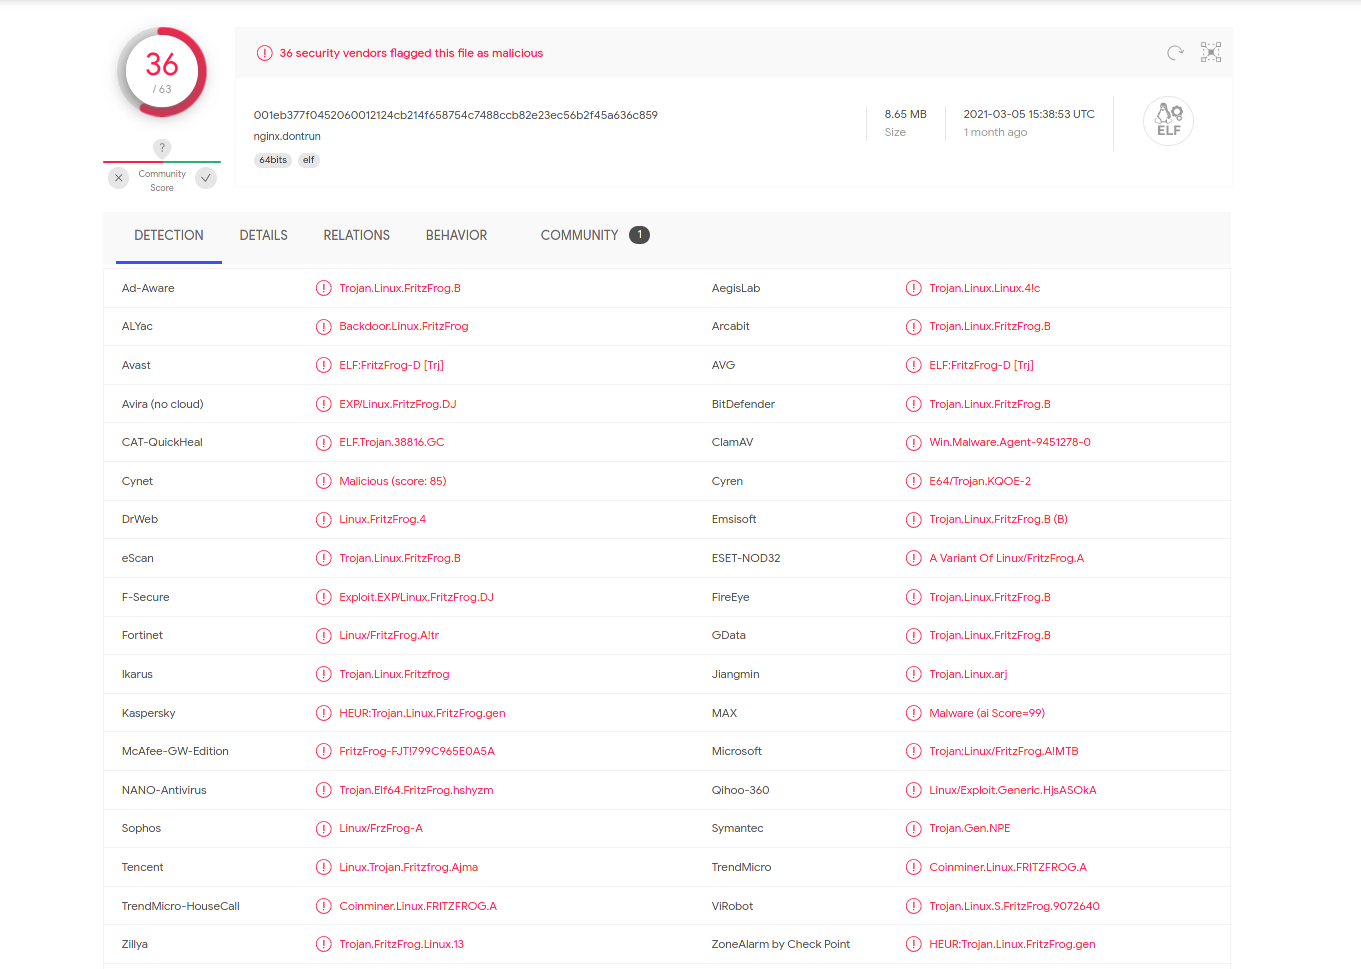
\includegraphics[width=\columnwidth]{pics/virustotal.png}
		\caption{Virustotal: Family Identification}
		\label{virustotal}
	\end{figure}
	The malware executable can be identified by submitting to Virustotal \cite{vt} as belonging to \textit{FritzFrog} malware family.

	\subsection{Section Headers}
	\begin{figure}[!htbp]% [!hb] forces image to be placed at that position
		\centering
		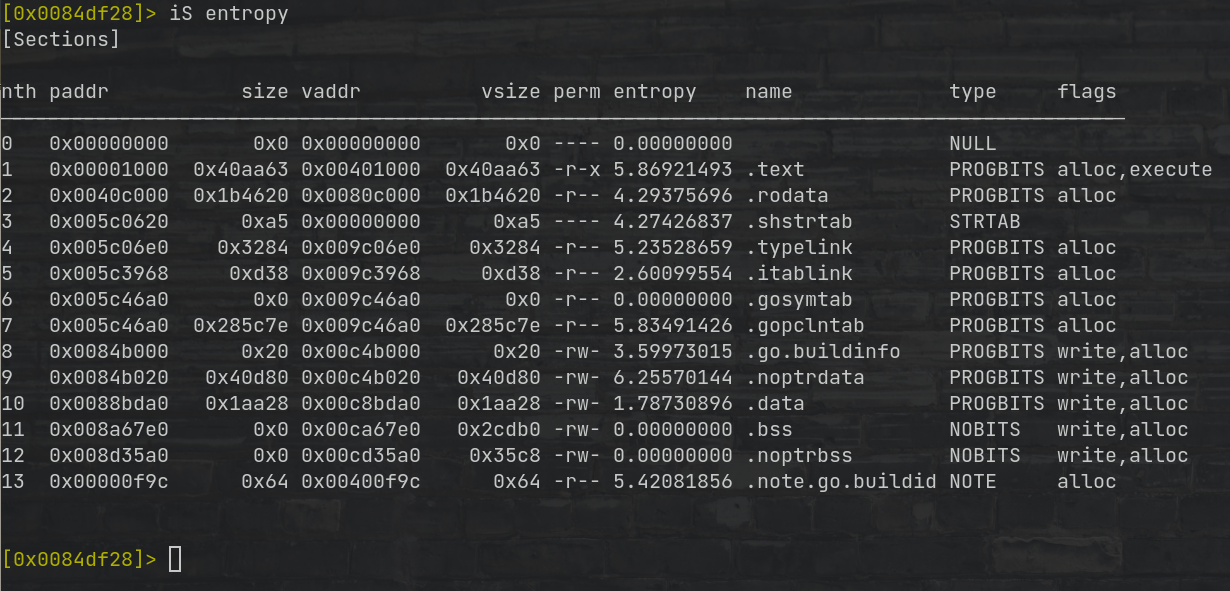
\includegraphics[width=\columnwidth]{pics/sections.png}
		\caption{Rizin: Binary Sections}
		\label{sections}
	\end{figure}
	The sections within the binary have expected entropy values and do not show any significant deviations from the norm of any regular go program (Fig. \ref{sections}).
	One interesting thing, though, is the \textit{.gopclntab} section \cite{pclntab}.
	This section contains contains mapping of individual functions with their line information from the original source files.
	This feature has been available since \textit{Go 1.2} and helps in getting author defined function names from the binary.
	Tools like \textit{Redress} \cite{redress} help in gathering the metadata.
	Also, \textit{Rizin} has been tested to perform similar metadata extraction during this analysis and a script for \textit{Ghidra} performs similar action \cite{gofunc}.

	\subsection{A case against Packing}
	The malware sample almost certainly shows no obfuscation techniques like packing or encryption.
	Not only the \textit{Go Lang} standard library functions, but the author generated function names can be recovered using the \textit{.gopclntab} section.
	Much of the \textit{peer-to-peer} functionality is visible including \textit{struct types} like \textit{main.Database}, \textit{main.DHGroup} and \textit{main.CryptoComm}.

	\subsection{Interesting Imports}
	Some of the imports from the \textit{Go} standard library as well as external packages are,
	\begin{itemize}
		\vspace{-0.7em}
		\item \textit{os/exec} which indicates towards command execution
		\item \textit{crypto/ssh} which indicates towards \textit{SSH} key exchange using \textit{DiffiHellman}, communication over \textit{SSH} channel etc.
		\item \textit{encoding/json and encoding/base64} which indicate \textit{JSON} as well as \textit{Base64} data serialization.
		\item \textit{net/http} which indicates some \textit{HTTP} functionality.
	\end{itemize}

	\subsection{Interesting Code Constructs}
	The following functions, established as user functions from \textit{Go .gopclntab} section are interesting,
	(functions missing sub-points when their name represents exactly what they do)
	\markdownInput{../impFeatures.md}

\newpage
\section{Dynamic Analysis}
	\subsection{Interesting Features}
	Following are some of the interesting features of the malware discovered on dynamic analysis,
	\begin{itemize}
		\vspace{-0.7em}
		\item On execution, it renames itself to \textit{nc} possibly in order to mimic \textit{GNU netcat} binary name.
		\item It opens up a \textit{TCP} port @1234 (Fig. \ref{ports}).
		\item On connecting to the port from another machine using \textit{Netcat}, it sends a Base64 encoded string which is different at every instance. This is most likely beginning of the \textit{Diffie-Hellman} key exchange process (Fig. \ref{pubkey}).
		\item On analyzing with \textit{strace} for system-calls, it exhibits multiple \textit{unlink} calls.
	\end{itemize}
\newpage

\section{Indicators of Compromise}
	\subsection{Host Based}
	Open \textit{TCP} port @\textbf{1234}

	\subsection{\textit{YARA} Rule}
	In case of unsuccessful copy from text below, use \cite{yara}.
		\lstinputlisting[language={},basicstyle=\tiny]{../rule.yar}

\newpage
\section{Appendix A: Screenshots}
\begin{figure}[!htbp]% [!hb] forces image to be placed at that position
	\centering
	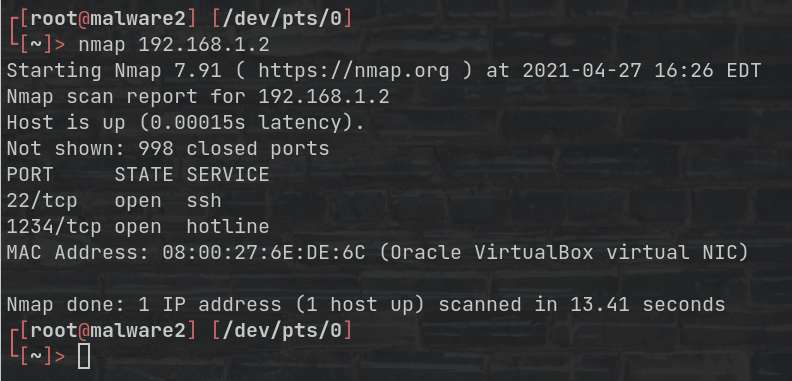
\includegraphics[width=\columnwidth]{pics/openPort.png}
	\caption{NMap: Open Ports on Victim machine}
	\label{ports}
\end{figure}

\begin{figure}[!htbp]% [!hb] forces image to be placed at that position
	\centering
	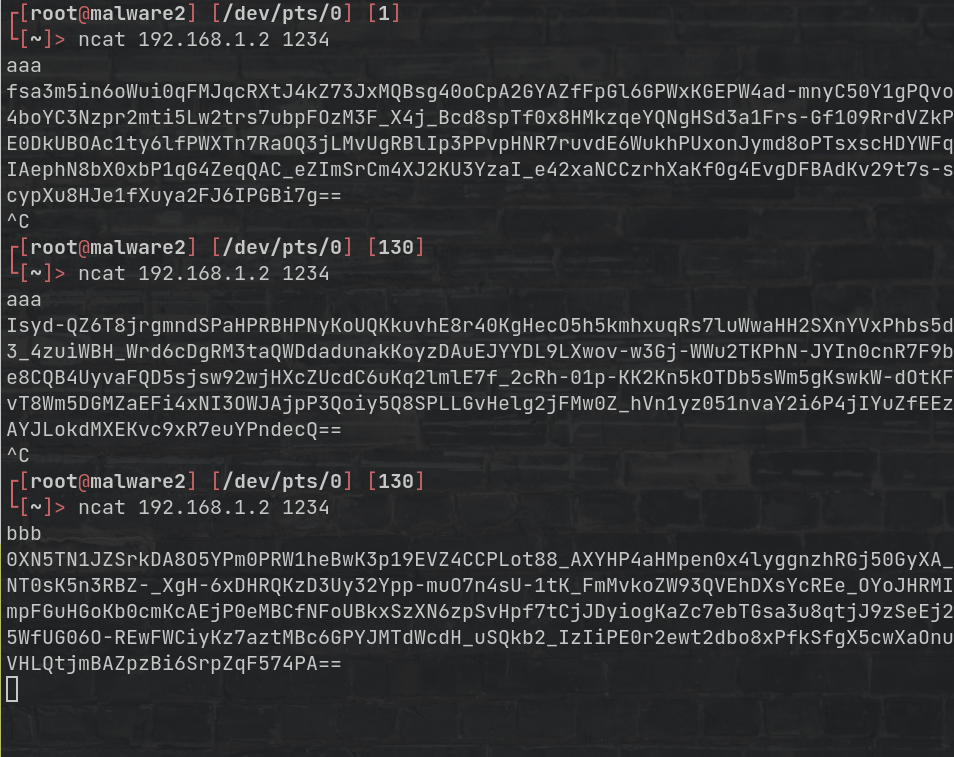
\includegraphics[width=\columnwidth]{pics/dhbegin.png}
	\caption{NCat: Base64 Encoded Key}
	\label{pubkey}
\end{figure}

\printbibliography
\end{document}